




%----------------------------------------------------------------------------------------


%%%%%%%%%%%%%%%%%%%%%%%
\section{Quantitative Epistemology}{Epistémologie Quantitative}

\label{app:sec:quantepistemo}


%----------------------------------------------------------------------------------------

\subsection{Algorithmic systematic review}{Revue systématique algorithmique}



\paragraph{Algorithm description}{Description de l'algorithme}



\bpar{
Let $A$ be an alphabet, $A^{\ast}$ corresponding words and $T = \cup_{k\in \mathbb{N}} {A^{\ast}}^k$ texts of finite length on it. A reference is for the algorithm a record with text fields representing title, abstract and keywords. Set of references at iteration $n$ will be denoted $\mathcal{C} \subset T^3$. We assume the existence of a set of keywords $\mathcal{K}_n$, initial keywords being $\mathcal{K}_0$. An iteration goes as follows :

\begin{enumerate}
\item A raw intermediate corpus $\mathcal{R}_n$ is obtained through a catalog request providing previous keywords $\mathcal{K}_{n-1}$.
\item Overall corpus is actualized by $\mathcal{C}_n = \mathcal{C}_{n-1} \cup \mathcal{R}_n$.
\item New keywords $\mathcal{K}_n$ are extracted from corpus through Natural Language Processing treatment, given a parameter $N_k$ fixing the number of keywords.
\end{enumerate}

The algorithm stops when corpus size becomes stable or a user-defined maximal number of iterations has been reached. Fig.~\ref{fig:quantepistemo:algo} shows the global workflow.
}{
Soit $A$ un alphabet (un ensemble arbitraire de symboles), $A^{\ast}$ les mots correspondants (chaînes de longueur finie sur l'alphabet). Les textes de longueur finie sur celui-ci sont donc $T = \cup_{k\in \mathbb{N}} {A^{\ast}}^k$. Ce qu'on nomme une référence est pour l'algorithme un enregistrement avec des champs textuels représentant le titre, le résumé et les mots-clés. L'ensemble de références à l'itération $n$ est ainsi noté $\mathcal{C}_n \subset T^3$ : il s'agit d'un sous-ensemble de triplets de textes. Nous supposons l'existence d'un ensemble de mots-clés $\mathcal{K}_n$, les mots-clés initiaux étant $\mathcal{K}_0$, spécifiés par l'utilisateur\footnote{On pourrait également partir d'un corpus $\mathcal{C}_0$, mais il s'agit plutôt de l'esprit de la méthodologie présentée dans la sous-section suivante. Nous nous en tiendrons ici pour cette exploration préliminaire en assumant le caractère arbitraire forcément biaisé de cette spécification. Le choix du corpus initial doit donc être fait en bonne connaissance des domaines existants, et fait nécessairement suite à la revue de littérature de~\ref{sec:modelingsa}.}. Une itération procède de la manière suivante :

\begin{enumerate}
\item Un corpus intermédiaire brut $\mathcal{R}_n$ est obtenu par une requête à un catalogue\footnote{Le catalogue est une fonction fournissant des références en réponse à une requête composée d'expression régulières de mots-clés. En pratique, nous utilisons le catalogue bibliographique en ligne Mendeley. La dépendance au catalogue devant sûrement introduire un biais que nous ne pouvons contrôler, une analyse de sensibilité ou le croisement de divers catalogues étant hors de propos pour cette analyse exploratoire.}
 auquel on fourni les mots-clés précédents $\mathcal{K}_{n-1}$.
\item Le corpus total est actualisé par $\mathcal{C}_n = \mathcal{C}_{n-1} \cup \mathcal{R}_n$.
\item Les nouveaux mot-clés $\mathcal{K}_n$ sont extraits du corpus par Traitement du Language Naturel (NLP), étant donné un paramètre fixé $N_k$ donnant le nombre de mot-clés extraits à cette étape.
\end{enumerate}

L'algorithme s'arrête quand la taille du corpus ne varie plus (l'expérience sur les requêtes testées montre pour celles-ci que le corpus ne contient plus de nouvelles références après un certain nombre d'itérations) ou quand un nombre maximal d'itérations défini par l'utilisateur est atteint. La figure~\ref{fig:quantepistemo:algo} synthétise le processus général.
}




\paragraph{Implementation}{Implémentation}


\bpar{
Because of the heterogeneity of operations required by the algorithm (references organisation, catalog requests, text processing), it was found a reasonable choice to implement it in Java. Source code is available on the Github repository of the project\footnote{at \texttt{https://github.com/JusteRaimbault/CityNetwork/tree/master/Models/QuantEpsitemo/AlgoSR}}. Catalog request, consisting in retrieving a set of references from a set of keywords, is done using the Mendeley software API \cite{mendeley} as it allows an open access to a large database. Keyword extraction is done by Natural Language Processing (NLP) techniques, following the workflow given in \cite{chavalarias2013phylomemetic}, calling a Python script that uses \cite{bird2006nltk}.
}{
De par l'hétérogénéité des opérations requises par l'algorithme (organisation des références, requêtes au catalogue, analyse textuelle), le language Java s'est présenté comme une alternative raisonnable. Le code source est disponible sur le dépôt ouvert du projet\footnote{à l'adresse \url{https://github.com/JusteRaimbault/CityNetwork/tree/master/Models/QuantEpistemo/AlgoSR}}. Les requêtes au catalogue, qui consistent à récupérer un ensemble de références à partir d'un ensemble de mots-clés, sont faites via l'API du logiciel Mendeley~\cite{mendeley} qui permet un accès ouvert à une base de données conséquente. L'extraction des mots-clés est effectuée par techniques d'Analyse Textuelle (NLP) selon le processus donné dans~\cite{chavalarias2013phylomemetic}, via un script Python qui utilise~\cite{bird2006nltk}.
}


\paragraph{Convergence and Sensitivity Analysis}{Convergence et analyse de sensibilité}


%\comment{(Florent) avec quels mots clés as tu validé empiriquement la convergence de l'algo?}

\bpar{
A formal proof of algorithm convergence is not possible as it will depend on the empirical unknown structure of request results and keywords extraction. We need thus to study empirically its behavior. Good convergence properties but various sensitivities to $N_k$ were found as presented in Fig.~\ref{fig:app:quantepistemo:sensitivity-algosr}. We also studied the internal lexical consistence of final corpuses as a function of keywords number. As expected, small number yields more consistent corpuses, but the variability when increasing stays reasonable.
}{
Une preuve formelle de convergence de l'algorithme n'est guère envisageable puisque qu'elle dépendra de la structure empirique inconnue des résultats de requête et d'extraction de mots-clés. Il est donc nécessaire d'étudier le comportement de l'algorithme de manière empirique. Comme présenté en Fig.~\ref{fig:app:quantepistemo:sensitivity-algosr}, l'algorithme a de bonnes propriétés de convergence mais diverses sensibilités à $N_k$. Nous étudions également la cohérence lexicale interne des corpus finaux et fonction du nombre de mots-clés. Comme attendu, des valeurs faibles produisent des corpus plus cohérents, mais la variabilité lorsque qu'elles augmentent reste raisonnable.
}



Nous prenons l'hypothèse la plus faible pour le paramètre $N_k=100$. En effet, plus $N_k$ est grand, moins le domaine exploré sera restreint, ce qui augmente les chances de recouvrement de deux corpus provenant de requêtes initiales différentes. Dans ce cas, une faible distance finale entre corpus sera plus significative pour des valeurs de $N_k$ grandes.


%%%%%%%%%%%%%%%%%%%%%%%%%%%%
\begin{figure}
%\includegraphics[width=\linewidth]{Figures/QuantEpistemo/explo}
%\includegraphics[width=\linewidth]{Figures/QuantEpistemo/lexicalConsistence_MeanSd}
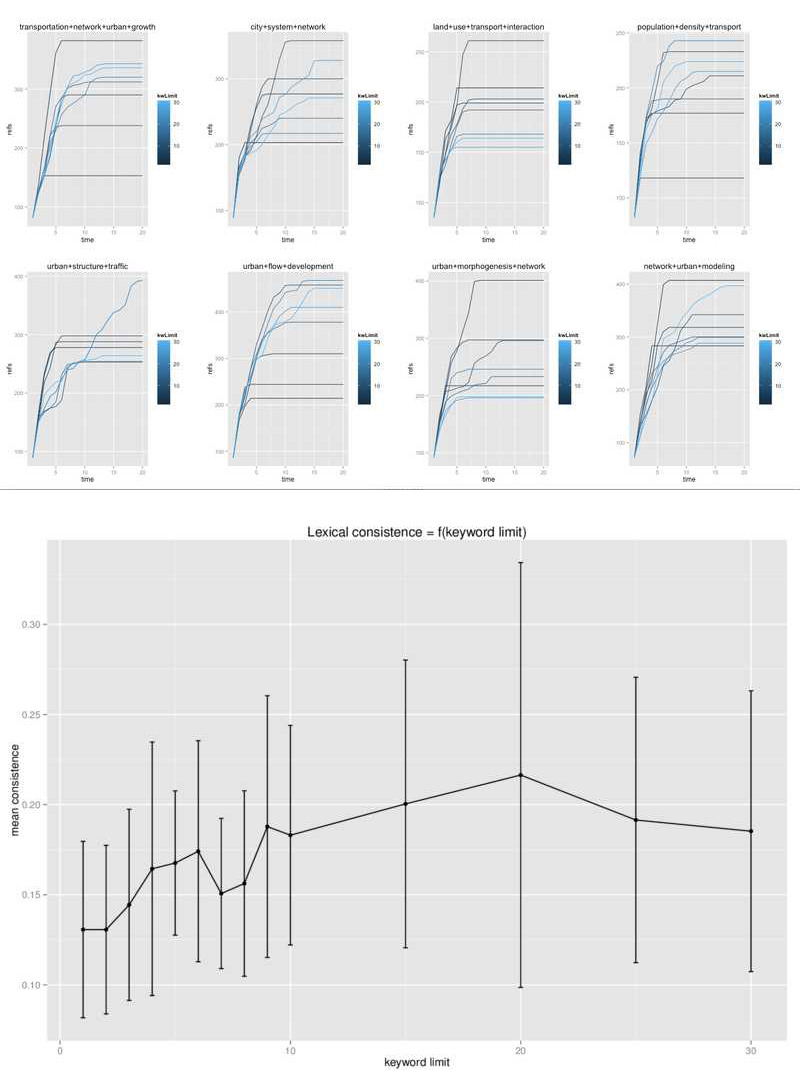
\includegraphics[width=\linewidth,height=0.85\textheight]{Figures/Final/A-quantepistemo-sensitivity-algosr.jpg}
\appcaption{Convergence and sensitivity analysis. Left : Plots of number of references as a function of iteration, for various queries linked to our theme (see further), for various values of $N_k$ (from 2 to 30). We obtain a rapid convergence for most cases, around 10 iterations needed. Final number of references appears to be very sensitive to keyword number depending on queries, what seems logical since encountered landscape should strongly vary depending on terms. Right : Mean lexical consistence and standard error bars for various queries, as a function of keyword number. Lexical consistence is defined though co-occurrences of keywords by, with $N$ final number of keywords, $f$ final step, and $c(i)$ co-occurrences in references, $k = \frac{2}{N(N-1)}\cdot \sum_{i,j \in \mathcal{K}_f}{\left| c(i) - c(j) \right|}$. The stability confirms the consistence of final corpuses.\label{fig:app:quantepistemo:sensitivity-algosr}}{\textbf{Convergence et analyse de sensibilité de l'algorithme de revue systématique.} (\textit{Haut}) Graphes des nombres de références en fonction de l'itération, pour différentes requêtes liées à notre thème, et pour différentes valeurs de $N_k$ (de 2 à 30, couleur). On obtient une convergence rapide dans la majorité des cas, autour de 10 itérations étant nécessaires. Le nombre final de références semble très sensible au nombre de mots-clés selon les requêtes, ce qui confirme une forte variabilité du paysage rencontré selon les termes. (\textit{Bas}) Consistence lexicale moyenne et déviation standard sur différentes requêtes, en fonction de $N_k$. La consistence lexicale est définie par les co-occurrences des mots-clés, comme $k = \frac{2}{N_k(N_k-1)}\cdot \sum_{i,j \in \mathcal{K}_f}{\left| c(i) - c(j) \right|}$, avec $f$ temps final, $c(i)$ co-occurrence des mots dans les références. La stabilisation confirme la consistence des corpus finaux.\label{fig:app:quantepistemo:sensitivity-algosr}}
\end{figure}
%%%%%%%%%%%%%%%%%%%%%%%%%%%%








%----------------------------------------------------------------------------------------

\subsection{Hypernetwork analysis}{Bibliométrie indirecte}


%%

\paragraph{Initial corpus}{Corpus initial}

Le tableau~\ref{tab:app:quantepistemo:corpus} donne la composition du corpus initial pour la construction du réseau de citation.

%%%%%%%%%%%%%
\begin{table}
\apptabcaption{\textbf{Composition of the initial corpus for the construction of the citation network.}\label{tab:app:quantepistemo:corpus}}{\textbf{Composition du corpus initial pour la construction du réseau de citation.}\label{tab:app:quantepistemo:corpus}}
	\begin{tabular}{|l|p{6cm}|l|}
	\hline
	Domaine & Titre & Référence \\\hline
	Sciences politiques & Les effets structurants du transport: mythe politique, mystification scientifique & \cite{offner1993effets} \\\hline 
	Interdisciplinaire & Réseaux et territoires-significations croisées & \cite{offner1996reseaux} \\\hline
	Géographie & Villes et réseaux de transport: des interactions dans la longue durée (France, Europe, Etats-Unis) & \cite{bretagnolle:tel-00459720} \\\hline
	Transports & Land-use transport interaction: state of the art & \cite{wegener2004land} \\\hline
	Économie & The co-evolution of land use and road networks & \cite{levinson2007co} \\\hline
	Économie & Modeling the growth of transportation networks: a comprehensive review & \cite{xie2009modeling} \\\hline
	Physique & Co-evolution of density and topology in a simple model of city formation & \cite{barthelemy2009co} \\\hline
	\end{tabular}
\end{table}
%%%%%%%%%%%%%




\paragraph{Sensitivity analysis}{Analyse de sensibilité}

L'analyse de sensibilité permettant de fixer les paramètres optimaux pour le réseau sémantique est montrée en Fig.~\ref{fig:app:quantepistemo:sensitivity}.

% degré non pondéré ? -> justifié dans le Cybergeo paper


%%%%%%%%%%%%%%%%%%
\begin{figure}
%\includegraphics[width=0.49\linewidth]{Figures/Quantepistemo/pareto-com-vertices}
%\includegraphics[width=0.49\linewidth]{Figures/Quantepistemo/pareto-modularity-vertices}\\
%\includegraphics[width=\linewidth]{Figures/Quantepistemo/sensitivity_freqmin0_normalized}
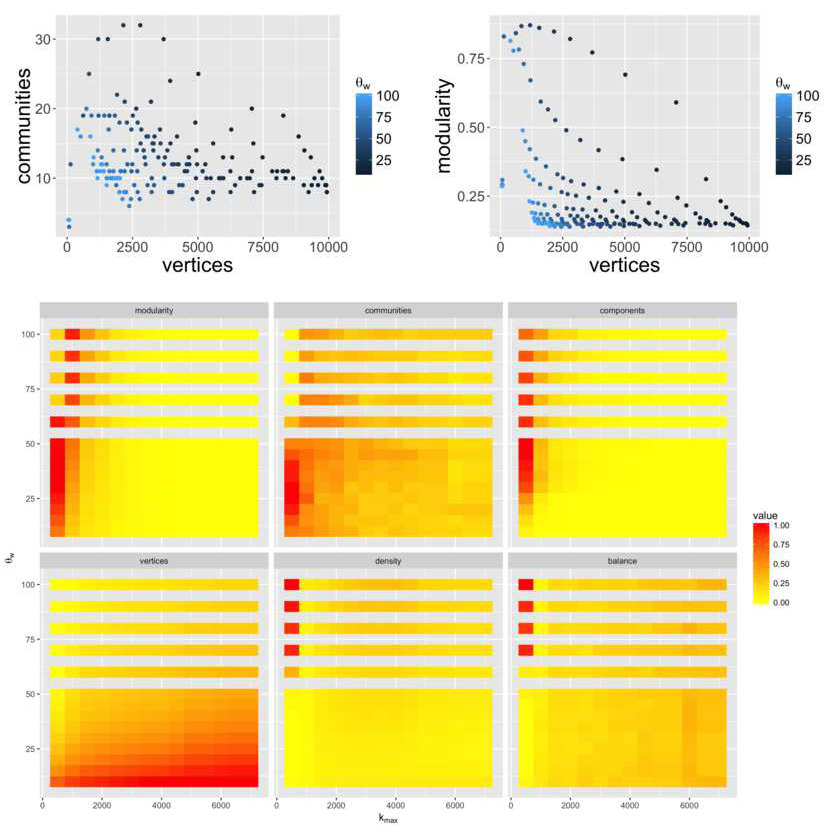
\includegraphics[width=\linewidth]{Figures/Final/A-quantepistemo-sensitivity.jpg}
\appcaption{\textbf{Sensitivity analysis of network indicators to filtering parameters.}\label{fig:app:quantepistemo:sensitivity}}{\textbf{Analyse de sensibilité des propriétés modulaires du réseau sémantique en fonction des paramètres de filtrage.} \textit{(Haut Gauche)} Front de Pareto du nombre de communauté et du nombre de sommets (deux objectifs à maximiser), la couleur donnant la valeur de $\theta_w$ ; \textit{(Haut Droite)} Front de Pareto de la modularité en fonction du nombre de sommets, pour $\theta_w$ variant ; \textit{(Bas)} Valeurs des objectifs possibles (modularité, nombre de communautés, nombre de composantes connexes, nombre de sommets, densité, équilibre de taille entre communautés), chaque objectif étant normalisé dans $\left[0;1\right]$, en fonction des paramètres $\theta_w$ et $k_{max}$.\label{fig:app:quantepistemo:sensitivity}}
\end{figure}
%%%%%%%%%%%%%%%%%%



\paragraph{Semantic Network}{Réseau Sémantique}

% Visualisation du réseau sémantique.

Une visualisation du réseau sémantique est donnée en Fig.~\ref{fig:app:quantepistemo:semanticnw}.

%%%%%%%%%%%%%%%%%%
\begin{figure}
%\includegraphics[width=\linewidth]{Figures/Quantepistemo/semantic}
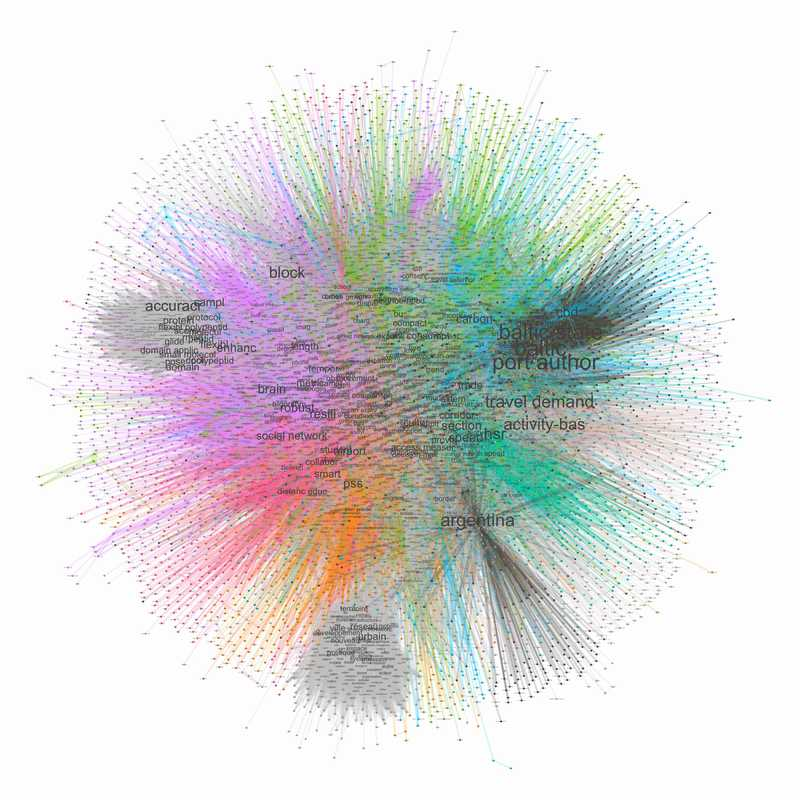
\includegraphics[width=\linewidth]{Figures/Final/A-quantepistemo-semanticnw.jpg}
\appcaption{\textbf{Semantic network of domains.} Network is constructed by co-occurrences of most relevant keywords. Filtering parameters are here taken according to the multi-objective optimization done in Fig.~\ref{fig:sensitivity}, i.e. $(k_{max}=,e_{th}=,f_{min},f_{max}=)$. The graph spatialization algorithm (Fruchterman-Reingold), despite its stochastic and path-dependent character, unveils information. A zoomable vectorial file (\texttt{.svg}) of the network is available as Supplementary Material.\label{fig:app:quantepistemo:semanticnw}}{\textbf{Réseau sémantique des domaines.} La couleur des liens donne la communauté et la taille des mots-clés est fixée par leur degré.\label{fig:app:quantepistemo:semanticnw}}
\end{figure}
%%%%%%%%%%%%%%%%%%





\stars





%----------------------------------------------------------------------------------------

\newpage

%%%%%%%%%%%%%%%%%%%%%%%
\section{Modelography}{Modélographie}

\label{app:sec:modelography}


%----------------------------------------------------------------------------------------



\subsection{Systematic Review Methodology}{Méthodologie de la revue systématique}


Pour le choix des mots-clés initiaux pour la constitution indirecte (via requête sémantique), une alternative possible est d'extraire les mots-clés pertinents par sous-communautés du réseau de citations, puis sélectionner les plus pertinents ensuite pour chaque domaine. Nous faisons le choix de les extraire sur le corpus complet, puis de les récupérer par sous-communautés ensuite. Pour un petit corpus, la deuxième option est plus souhaitable, puisque la notion de pertinence moins importante que pour des très grands corpus, ou certains mots pertinents pourront être noyés et des moins pertinents ressortir de manière fortuite. En d'autre termes, la méthode de selection des mots-clés parait plus robuste sur des petits corpus, comme le suggère la comparaison de cette application avec celle faite sur le journal Cybergeo et celle faite sur le corpus de brevets (voir~\ref{app:sec:patentsmining}).

%(mentionner Patents et Cybergeo, ressemblances et différences).




% random stuff removed manual screening 
%computer sci, neurosci, geology, chem/bio terrorism WTF ? , theoretical physics, eco des orgs, socio (aids ethiopia ?), target tracking, rice storage culinary qual, bulimic, smart cities, bullshit territorialité Die, chinese migrants !, chinese tourist HongKong, papier CN desakota (cité migrdyn), health, hydrology, paysage hautes corbières, musical implication network, finance capitalism, produit territoire pomme des alpes, mobilité sociale, vibration pont hsr, ontological knowledge industri., signal processing, anger/agression, flocks/schools, friendship and mobility, consumer brand,  aghion ? , colorectal cancer texas, lidar urban, mediteranean cities, sun and sand tourism, gender car use, gold rush movies, urban informatics, "best outside US", badger, robots beacon, milieux innovateurs, politique univ villes la rochelle etc, cosmology, economie de la qualité,  handbook adult resilience, stock price, archeo chefferie, speculative urb, Mendoza arg, subway platfrom ventilation, magaliths, crowding HK light rail !, terrritoire familiaux naples classes sup, performing arts series, sncf tunnel rig, china snow disaster; fabriq rue paris 19e, geopol inuit, espace public beyrouth, greenway., desire named streetcar, jeddah, french competitino rail myth, Equip the warrior instead of manning the equipment, aparheid namibia, baselIII finance, tokyo, espace transfrtontalier, transport proteins !, hedonic rail road noise, croissance syst urbain loi metropol, maritime nw indonesia, eco sociale au quebec, first world urban activism, hybrid.. , gentrif nvel urba, [before] Estimation of local spatial scale : otpicians !, stations de montange, street gang sptail pattern LA, SFI adress !, bogota BRT, transport noise, brussel urban geology, drosohiplia embryo


\subsubsection{Article screening}{Première revue du corpus}

Les méthodes utilisées ne permettent pas de s'affranchir d'un ``bruit'', c'est à dire d'article ne relevant a priori pas même de loin à la thématique. Nous avons obtenu par exemple des articles aussi divers qu'incongrus sur le genre et l'usage de la voiture, le cancer colorectal au Texas, la mécanique des vibrations au passage d'un train à grande vitesse, le transport des protéines dans la cellule, l'espace public à Beyrouth, les motifs spatiaux des \emph{street gangs} à Los Angeles, la géologie urbaine à Bruxelles. Cela confirme que l'étape de filtrage manuel est essentielle.

Ce bruit peut être du par exemple à :
\begin{itemize}
	\item Des citations effectives pour diverses raisons, mais n'ayant que peu de pertinence dans l'article citant.
	\item Du bruit intrinsèque à la recherche par mots-clés.
	\item Des erreurs de classification du catalogue.
\end{itemize}



\subsubsection{Remarks on manual screening}{Remarques sur la classification manuelle}

Lors de la classification manuelle opérée lors de l'inspection des résumés, les points suivants ressortent :

\begin{itemize}
	\item Les disciplines ``a priori'' sont jugées par le journal dans lequel l'article a été publié. En l'occurence, nous opérons les choix particuliers suivants (pour d'autres journaux comme des journaux de physique il n'y a pas d'ambiguïté) : Journal of Transport Geography, Environment and Planning B : geography ; Journal of Transport and Land-Use, Transportation Research : Transportation.
	\item La géographie en notre sens inclut l'urbanisme et les études urbaines si celles-ci ne sont pas trop proches de la planification (urbain durable par exemple).
\end{itemize}






\subsection{Meta-analysis}{Meta-analyse}

Nous donnons ici les résultats numériques complets des analyses statistiques reliant caractéristiques de modèles et variables explicatives.


\subsubsection{Variables values}{Modalités des variables}

Rappelons ici les variables utilisées dans la méta-analyse et leur modalités. Celles-ci sont :

\begin{itemize}
	\item Type de modèle (\texttt{TYPE}) : strong, territory, network.
	\item Année de publication (\texttt{YEAR}), nombre entier.
	\item Communauté de citation (\texttt{CITCOM}), définies par le réseau de citations : Accessibility, Geography, Infra Planning, LUTI, Networks, TOD.
	\item Discipline a priori (\texttt{DISCIPLINE}) : biology, computer science, economics, engineering, environment, geography, physics, planning, transportation.
	\item Communauté sémantique (\texttt{SEMCOM}) : brt, complex networks, hedonic, hsr, infra planning, networks, tod.
	\item Méthodologie utilisée : ca (\emph{Cellular Automaton}), eq (équations analytiques), map (cartographie), mas (\emph{Multi-agent simulation}), ro (recherche opérationnelle), sem (\emph{Structural Equation Modeling}), sim (simulation), stat (statistiques).
	\item Indice d'interdisciplinarité (\texttt{INTERDISC}) : réel dans $[0,1]$.
	\item Echelle temporelle (\texttt{TEMPSCALE}) : donnée en année, vaut 0 pour les analyses statiques.
	\item Echelle spatiale (\texttt{SPATSCALE}) : continent (10000), country (1000), region (100), metro (10). Ces modalités sont transformées numériquement en km par les valeurs données entre parenthèses (échelles stylisées).
\end{itemize}

%La variable d'équilibre (modèles supposant un équilibre ou non) n'a pas pu être construite.



\subsubsection{Model selection}{Sélection des modèles}

Concernant la sélection des modèles, celle-ci n'est pas opérée en critère unique, de par le faible nombre d'observations pour certains modèles, mais par l'optimisation au sens de Pareto des objectifs contradictoires de l'ajustement ($R^2$ ajusté, à maximiser) et du sur-ajustement (critère d'Akaike corrigé AICc, à minimiser), tout en contrôlant le nombre de points d'observation. La Fig.~\ref{fig:app:quantepistemo:regressions} donne pour chaque variable à expliquer la localisation de l'ensemble des modèles potentiels dans l'espace des objectifs, ainsi que le nombre d'observations correspondantes. Pour l'interdisciplinarité, deux nuages de points correspondent à des compromis différents, et nous sélectionnons les deux modèles optimaux (un pour chaque nuage). Pour l'échelle d'espace, nous postulons un $R^2$ positif, et un seul modèle optimal émerge alors. Pour l'échelle de temps, on a comme pour l'interdisciplinarité deux modèles compromis. Enfin, pour l'année, le gain en AICc entre les deux optimaux potentiels est négligeable en comparaison à la perte en $R^2$, et nous sélectionnons donc le modèle optimal tel que $R^2>0.25$ et AICc$<600$. Les résultats des modèles sont donnés par la suite.


%%%%%%%%%%%%%%
\begin{figure}
%\includegraphics[width=0.48\linewidth]{Figures/QuantEpistemo/lm_adjr2-aicc_INTERDISC.pdf}
%\includegraphics[width=0.48\linewidth]{Figures/QuantEpistemo/lm_adjr2-aicc_SPATSCALE.pdf}
%\includegraphics[width=0.48\linewidth]{Figures/QuantEpistemo/lm_adjr2-aicc_TEMPSCALE.pdf}
%\includegraphics[width=0.48\linewidth]{Figures/QuantEpistemo/lm_adjr2-aicc_YEAR.pdf}
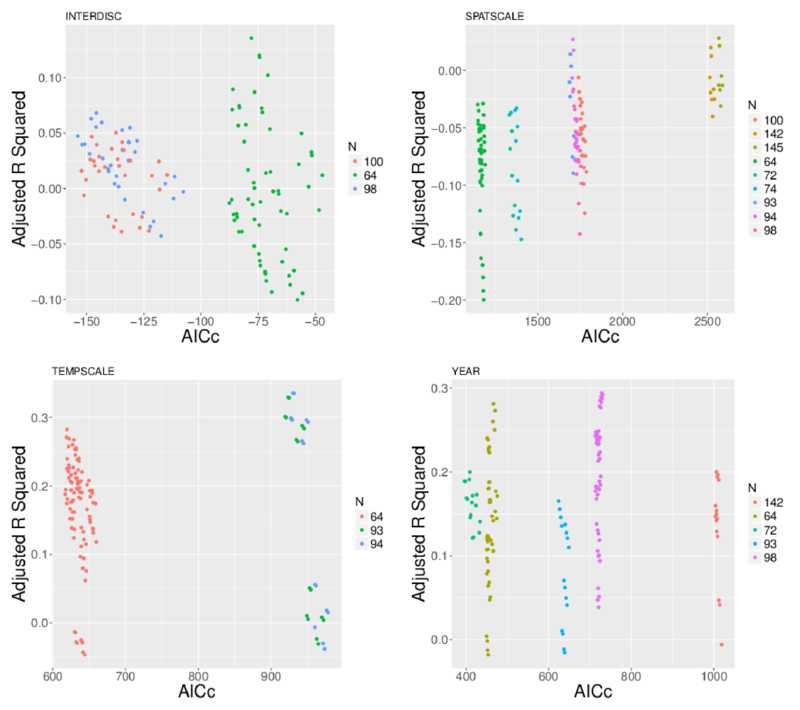
\includegraphics[width=\linewidth]{Figures/Final/A-quantepistemo-regressions.jpg}
\appcaption{\textbf{Multi-objective selection of linear models.}\label{fig:app:quantepistemo:regressions}}{\textbf{Sélection multi-objectif des modèles linéaires.} Pour chaque variable à expliquer, nous représentons la position de l'ensemble des modèles linéaires dans l'espace des objectifs (critère d'Akaike corrigé AICc et $R^2$ ajusté). La couleur des points donne le nombre d'observations.\label{fig:app:quantepistemo:regressions}}
\end{figure}
%%%%%%%%%%%%%%



\subsubsection{Model fitting}{Ajustement des modèles}


\paragraph{Interdisciplinarity}{Interdisciplinarité}


L'interdisciplinarité est ajustée selon les modèles linéaires présentés en Table~\ref{tab:app:modelography:interdisc}.



%%%%%%%%%%%%%%
\begin{table}%[!htbp] \centering 
  \apptabcaption{\label{tab:app:modelography:interdisc}}{\textbf{Modèles linéaires pour l'interdisciplinarité.}\label{tab:app:modelography:interdisc}}
\begin{tabular}{@{\extracolsep{5pt}}lcc} 
\footnotesize
\\[-1.8ex]\hline 
\hline \\[-1.8ex] 
 %& \multicolumn{2}{c}{\textit{Dependent variable:}} \\ 
%\cline{2-3} 
\\[-1.8ex] & \multicolumn{2}{c}{INTERDISC} \\ 
\\[-1.8ex] & (1) & (2)\\ 
\hline \\[-1.8ex] 
 YEAR & $-$0.004 ($-$0.008, $-$0.00002), p = 0.055$^{*}$ & $-$0.002 ($-$0.005, 0.0001), p = 0.061$^{*}$ \\ 
  TEMPSCALE & $-$0.0003 ($-$0.001, 0.001), p = 0.615 &  \\ 
  DISCIPLINEengineering & 0.144 ($-$0.082, 0.371), p = 0.218 &  \\ 
  DISCIPLINEenvironment & 0.092 ($-$0.132, 0.316), p = 0.425 &  \\ 
  DISCIPLINEgeography & 0.036 ($-$0.043, 0.114), p = 0.378 &  \\ 
  DISCIPLINEphysics & $-$0.103 ($-$0.287, 0.080), p = 0.275 &  \\ 
  DISCIPLINEplanning & $-$0.047 ($-$0.135, 0.041), p = 0.30 &  \\ 
  DISCIPLINEtransportation & 0.062 ($-$0.025, 0.149), p = 0.169 &  \\ 
  TYPEstrong &  & $-$0.026 ($-$0.134, 0.081), p = 0.633 \\ 
  TYPEterritory &  & 0.044 ($-$0.026, 0.114), p = 0.222 \\ 
  SEMCOMcomplex networks &  & $-$0.217 ($-$0.522, 0.087), p = 0.166 \\ 
  SEMCOMhedonic & $-$0.179 ($-$0.407, 0.049), p = 0.130 & $-$0.184 ($-$0.400, 0.032), p = 0.100$^{*}$ \\ 
  SEMCOMhsr & $-$0.100 ($-$0.361, 0.162), p = 0.459 & $-$0.122 ($-$0.357, 0.112), p = 0.309 \\
  SEMCOMinfra planning & $-$0.032 ($-$0.273, 0.209), p = 0.797 & $-$0.096 ($-$0.321, 0.128), p = 0.404  \\ 
  SEMCOMnetworks & $-$0.038 ($-$0.272, 0.195), p = 0.750 & $-$0.107 ($-$0.324, 0.109), p = 0.335 \\ 
  SEMCOMtod & $-$0.105 ($-$0.332, 0.121), p = 0.366 & $-$0.152 ($-$0.364, 0.060), p = 0.165 \\ 
  Constant & 8.962 (0.776, 17.147), p = 0.037$^{**}$ & 5.531 (0.575, 10.487), p = 0.032$^{**}$ \\
 \hline \\[-1.8ex] 
Observations & 64 & 98 \\ 
R$^{2}$ & 0.314 & 0.155 \\ 
Adjusted R$^{2}$ & 0.136 & 0.068 \\ 
Residual Std. Error & 0.109 (df = 50) & 0.107 (df = 88) \\ 
F Statistic & 1.761$^{*}$ (df = 13; 50) & 1.789$^{*}$ (df = 9; 88) \\ 
\hline 
\hline \\[-1.8ex] 
\textit{Note:}  & \multicolumn{2}{r}{$^{*}$p$<$0.1; $^{**}$p$<$0.05; $^{***}$p$<$0.01} \\ 
\end{tabular} 
\end{table} 
%%%%%%%%%%%%%%




\paragraph{Spatial scale}{Echelle d'espace}


L'échelle spatiale est ajustée selon le modèle linéaire dont l'ajustement est donné en Table~\ref{tab:app:modelography:spatscale}.

%\[
%\begin{split}
%	SPATSCALE \sim & YEAR+CITCOM+TYPE+TEMPSCALE+ \\
%	& FMETHOD+DISCIPLINE+INTERDISC+SEMCOM
%\end{split}
%\]


%%%%%%%%%%%%%
\begin{table}%[!htbp] \centering 
  \apptabcaption{\label{tab:app:modelography:spatscale}}{\textbf{Modèle linéaire pour l'échelle spatiale.}\label{tab:app:modelography:spatscale}}
\begin{tabular}{@{\extracolsep{5pt}}lc} 
\\[-1.8ex]\hline 
\hline \\[-1.8ex] 
 %& \multicolumn{1}{c}{\textit{Dependent variable:}} \\ 
%\cline{2-2} 
\\[-1.8ex] & SPATSCALE \\ 
\hline \\[-1.8ex] 
 TEMPSCALE & $-$5.179 ($-$16.259, 5.901) \\ 
  & p = 0.363 \\ 
  DISCIPLINEengineering & $-$154.461 ($-$3,003.326, 2,694.405) \\ 
  & p = 0.916 \\ 
  DISCIPLINEenvironment & $-$5.878 ($-$3,977.974, 3,966.219) \\ 
  & p = 0.998 \\ 
  DISCIPLINEgeography & 1,445.457 (389.349, 2,501.565) \\ 
  & p = 0.009$^{***}$ \\ 
  DISCIPLINEphysics & 292.559 ($-$2,717.659, 3,302.777) \\ 
  & p = 0.850 \\ 
  DISCIPLINEplanning & $-$143.554 ($-$1,361.357, 1,074.249) \\ 
  & p = 0.818 \\ 
  DISCIPLINEtransportation & 568.329 ($-$606.167, 1,742.826) \\ 
  & p = 0.346 \\ 
  Constant & 235.357 ($-$458.201, 928.914) \\ 
  & p = 0.508 \\ 
 \hline \\[-1.8ex] 
Observations & 94 \\ 
R$^{2}$ & 0.100 \\ 
R$^{2}$ ajusté & 0.027 \\ 
Erreur Std. Résiduelle & 1,995.272 (df = 86) \\ 
Statistique F & 1.369 (df = 7; 86) \\ 
\hline 
\hline \\[-1.8ex] 
\textit{Note:}  & \multicolumn{1}{r}{$^{*}$p$<$0.1; $^{**}$p$<$0.05; $^{***}$p$<$0.01} \\ 
\end{tabular} 
\end{table} 
%%%%%%%%%%%%%






\paragraph{Time scale}{Echelle de temps}

L'échelle de temps est ajustée selon les modèles linéaires présentés en Table~\ref{tab:app:modelography:tempscale}.

%\[
%\begin{split}
%	TEMPSCALE \sim & YEAR+CITCOM+TYPE+SPATSCALE+FMETHOD\\
%	& +DISCIPLINE+INTERDISC+SEMCOM
%\end{split}
%\]

%%%%%%%%%
\begin{table}%[!htbp] \centering 
    \apptabcaption{\label{tab:app:modelography:tempscale}}{\textbf{Modèles linéaires pour l'échelle temporelle.}\label{tab:app:modelography:tempscale}}
\begin{tabular}{@{\extracolsep{5pt}}lcc} 
\\[-1.8ex]\hline 
\hline \\[-1.8ex] 
% & \multicolumn{2}{c}{\textit{Dependent variable:}} \\ 
%\cline{2-3} 
\\[-1.8ex] & \multicolumn{2}{c}{TEMPSCALE} \\ 
\\[-1.8ex] & (1) & (2)\\ 
\hline \\[-1.8ex] 
 YEAR & 0.674 ($-$0.294, 1.643) &  \\ 
  & p = 0.179 &  \\ 
  TYPEstrong &  & 100.271 (58.312, 142.230) \\ 
  &  & p = 0.00002$^{***}$ \\ 
  TYPEterritory & $-$38.933 ($-$64.249, $-$13.617) & $-$14.988 ($-$37.411, 7.435) \\ 
  & p = 0.004$^{***}$ & p = 0.194 \\ 
  DISCIPLINEengineering & $-$52.107 ($-$110.950, 6.735) & $-$9.609 ($-$55.841, 36.624) \\ 
  & p = 0.089$^{*}$ & p = 0.685 \\ 
  DISCIPLINEenvironment & 17.110 ($-$37.350, 71.569) & 17.886 ($-$45.319, 81.090) \\ 
  & p = 0.541 & p = 0.581 \\ 
  DISCIPLINEgeography & 3.640 ($-$15.364, 22.644) & 9.126 ($-$7.590, 25.843) \\ 
  & p = 0.709 & p = 0.288 \\ 
  DISCIPLINEphysics & 46.879 (0.638, 93.120) & 77.897 (28.225, 127.570) \\ 
  & p = 0.053$^{*}$ & p = 0.003$^{***}$ \\ 
  DISCIPLINEplanning & 1.304 ($-$19.336, 21.945) & 4.553 ($-$14.865, 23.971) \\ 
  & p = 0.902 & p = 0.648 \\ 
  DISCIPLINEtransportation & $-$14.718 ($-$34.978, 5.543) & 8.753 ($-$9.864, 27.371) \\ 
  & p = 0.161 & p = 0.360 \\ 
  INTERDISC & 2.357 ($-$59.200, 63.915) &  \\ 
  & p = 0.941 &  \\ 
  Constant & $-$1,305.126 ($-$3,252.499, 642.247) & 22.103 ($-$0.951, 45.156) \\ 
  & p = 0.195 & p = 0.064$^{*}$ \\ 
 \hline \\[-1.8ex] 
Observations & 64 & 94 \\ 
R$^{2}$ & 0.385 & 0.393 \\ 
Adjusted R$^{2}$ & 0.282 & 0.336 \\ 
Residual Std. Error & 26.984 (df = 54) & 31.747 (df = 85) \\ 
F Statistic & 3.755$^{***}$ (df = 9; 54) & 6.871$^{***}$ (df = 8; 85) \\ 
\hline 
\hline \\[-1.8ex] 
\textit{Note:}  & \multicolumn{2}{r}{$^{*}$p$<$0.1; $^{**}$p$<$0.05; $^{***}$p$<$0.01} \\ 
\end{tabular} 
\end{table} 
%%%%%%%%%



\paragraph{Year}{Année}

L'année de publication est ajustée selon le modèle linéaire dont l'ajustement est donné en Table~\ref{tab:app:modelography:year}.

%%%%%%%%%%%%%%
\begin{table}%[!htbp]
  \apptabcaption{\label{tab:app:modelography:year}}{\textbf{Modèle linéaire pour l'année de publication.}\label{tab:app:modelography:year}}
\begin{tabular}{@{\extracolsep{5pt}}lc} 
\footnotesize
\\[-1.8ex]\hline 
\hline \\[-1.8ex] 
% & \multicolumn{1}{c}{\textit{Dependent variable:}} \\ 
%\cline{2-2} 
\\[-1.8ex] & YEAR \\ 
\hline \\[-1.8ex] 
 TYPEterritory & 10.898 (3.045, 18.750), p = 0.010$^{***}$ \\ 
  TEMPSCALE & 0.035 ($-$0.033, 0.103), p = 0.320 \\ 
  FMETHODeq & $-$6.224 ($-$20.162, 7.714), p = 0.387 \\ 
  FMETHODmap & 4.747 ($-$7.595, 17.089), p = 0.456 \\ 
  FMETHODro & 6.128 ($-$11.694, 23.950), p = 0.504 \\ 
  FMETHODsem & 1.009 ($-$16.659, 18.676), p = 0.912 \\ 
  FMETHODsim & 5.153 ($-$6.809, 17.114), p = 0.404 \\ 
  FMETHODstat & $-$0.357 ($-$10.925, 10.211), p = 0.948 \\ 
  DISCIPLINEengineering & 13.486 ($-$7.238, 34.210), p = 0.210 \\ 
  DISCIPLINEenvironment & $-$3.668 ($-$21.605, 14.269), p = 0.691 \\ 
  DISCIPLINEgeography & 1.121 ($-$4.528, 6.769), p = 0.700 \\ 
  DISCIPLINEphysics & 3.392 ($-$8.461, 15.245), p = 0.578 \\ 
  DISCIPLINEplanning & $-$2.850 ($-$8.873, 3.173), p = 0.359 \\ 
  DISCIPLINEtransportation & 5.503 (0.006, 11.000), p = 0.057$^{*}$ \\ 
  INTERDISC & $-$12.876 ($-$29.567, 3.815), p = 0.138 \\ 
  SEMCOMhedonic & $-$5.769 ($-$19.931, 8.393), p = 0.430 \\ 
  SEMCOMhsr & 6.135 ($-$9.889, 22.159), p = 0.458 \\ 
  SEMCOMinfra planning & $-$4.123 ($-$18.910, 10.663), p = 0.588 \\ 
  SEMCOMnetworks & 4.711 ($-$9.736, 19.158), p = 0.527 \\ 
  SEMCOMtod & $-$1.653 ($-$15.837, 12.532), p = 0.821 \\ 
  Constant & 2,004.945 (1,981.531, 2,028.359), p = 0.000$^{***}$ \\ 
 \hline \\[-1.8ex] 
Observations & 64 \\ 
R$^{2}$ & 0.510 \\ 
Adjusted R$^{2}$ & 0.281 \\ 
Residual Std. Error & 6.617 (df = 43) \\ 
F Statistic & 2.234$^{**}$ (df = 20; 43) \\ 
\hline 
\hline \\[-1.8ex] 
\textit{Note:}  & \multicolumn{1}{r}{$^{*}$p$<$0.1; $^{**}$p$<$0.05; $^{***}$p$<$0.01} \\ 
\end{tabular} 
\end{table} 
%%%%%%%%%%%%%%









